\section{Convolutional Neural Networks}
\subsection{Introduction}
\emph{Convolutional Neural Networks} (CNNs) is a class of models widely used in computer vision. While Fully Connected Neural Networks are very powerful machine learning models, they do not respect the 2D spatial structure of the input images. For instance, training a Multilayer Perceptron on a dataset of $32\times 32$ images required the model to start with a \texttt{Flatten} layer, that reshaped matrix images of size \texttt{(32, 32)} to flattened vectors of size \texttt{(1024, 1)}. Similarly, different color channels were handled separately, reshaping tensor images of dimensions \texttt{(32, 32, 3)} to \texttt{(3072, 1)}.

\begin{figure}[H]
    \centering
    \begin{tikzpicture}
        \newcommand{\randint}{
            \pgfmathsetmacro{\temp}{random(0, 1)}
            \temp
        }
        \fill[orange!60] (-1.9, -1.9) rectangle (1.9, 1.9);
        \matrix [
            matrix of math nodes,
            nodes={
                minimum size=1em,
                outer sep=0pt,
                inner sep=0,line
                width=0.5pt,
                append after command={
                    \pgfextra{\draw[thick]
                    ($(\tikzlastnode.north west)+(-0.4em,+0.4em)$)
                    rectangle ($(\tikzlastnode.south east)+(0.4em,-0.4em)$);}
                }
            },
            nodes in empty cells,
            column sep=-0.5pt,
            row sep=-0.5pt
        ]
        {
            \randint & \randint & \randint & \randint & \randint \\
            \randint & \randint & \randint & \randint & \randint \\
            \randint & \randint & \randint & \randint & \randint \\
            \randint & \randint & \randint & \randint & \randint \\
            \randint & \randint & \randint & \randint & \randint \\
        };

        \draw[<->, thick] (-1.9, -2.1) -- (1.9, -2.1) node[below, pos=0.5] {$32$};
        \draw[<->, thick] (-2.1, -1.9) -- (-2.1, 1.9) node[left, pos=0.5] {$32$};

        \draw[-, thick] (2.1, 0) -- (5, 0) node[above, pos=0.5] {Flatten};
        \draw[-, thick] (5, 2) -- (5, -2);

        \draw[->, thick] (5, 2) -- (5.2, 2);
        \draw[->, thick] (5, -2) -- (5.2, -2);

        \foreach \y in {-2, -1.5, ..., 2}
        {
           \node[circle,draw,thick,fill=orange!60] at (5.5, \y) {};
        }

        \draw[<->, thick] (6, 2.1) -- (6, -2.1) node[right, pos=0.5] {$1024$};
    \end{tikzpicture}
    \caption{Flatten layer breaking the spatial strucutre of input data}
\end{figure}

CNNs introduce new operators taking advantage of the spatial structure of the input data, while remaining compatible with automatic differentiation. While MLPs build the basic blocks of Deep Neural Networks using Fully-Connected Layers and Activation Layers, this chapter will introduce three new types of layers: \emph{Convolution Layers}, \emph{Pooling Layers}, and \emph{Normalization}.

\subsection{Convolution Layers}
Similarly to Fully-Connected Layers, \emph{Convolution Layers} have learnable weights, but also have the particularity to respect the spatial information.

\subsubsection{Input shape}
A Fully-Connected layer (also known as Linear layer) receives some flattened vector and outputs another vector:
\begin{figure}[H]
    \centering
    \begin{tikzpicture}
        \node at (-7, 0.7) {Input};
        \parallelepiped{(-4, 0, 0)}{6}{.5}{.5}{$3072$}{$1$}{}{blue!20}

        \draw[->, thick] (-3.4, -.2) -- (0.2, -.2) node[above, pos=.5] {$Wx$} node[below, pos=.5] {$W\in\mathscr{M}_{10,3072}(\R)$};

        \node at (2.5, .7) {Output};
        \parallelepiped{(4, 0, 0)}{3}{.5}{.5}{$10$}{$1$}{}{red!30}
    \end{tikzpicture}
    \caption{Fully-Connected Layer}
\end{figure}

Instead, a CNN takes as an input a 3D volume: for instance, an image can be represented as a tensor of shape $3\times32\times32$, the first dimension being the number of channels (red, green, blue), and the other two being the width and height of the image.

\subsubsection{Kernels}
The convolutional layer itself consists of small kernels (also called filters) used to \emph{convolve} with the image, that is sliding over it spatially, and computing the dot products at each possible location.
\begin{definition}[Kernel]
    A \emph{kernel} (or \emph{filter}) is a tensor of dimensions $D\times K\times K$, where $D$ is the number of channels (or \say{depth}) of the input, and $K$ is a parameter called \emph{kernel size}.
\end{definition}

\begin{definition}[Convolution of two matrices]
    Given two matrices $A=(a_{i, j})_{i, j}$ and $B=(b_{i, j})_{i, j}$ in $\mathscr{M}_{m, n}(\R)$, the \emph{convolution of $A$ and $B$}, noted $A*B\in\R$, is the following:
    \begin{equation}
        A*B = \sum_{i=1}^m \sum_{j=1}^n a_{(m-i+1), (n-j+1)} \cdot b_{i, j}
    \end{equation}
    This corresponds to the dot product in the space $\mathscr{M}_{m, n}(\R)$.
\end{definition}

\begin{definition}[Kernel convolution]
    An input of shape $C\times H\times W$ can be processed by a kernel of shape $C\times K\times K$ by computing at each possible spatial position the convolution between the kernel and the submatrix of the input.
    \begin{figure}[H]
        \centering
        \begin{tikzpicture}[scale=.5]
            \tdplotsetmaincoords{70}{140}
            \begin{scope}[tdplot_main_coords,canvas is yz plane at x=0]
                \draw[fill=red!50, thick] (19, 8) rectangle (20, 9);
                \draw (18,4) grid (24, 10);

                \draw[thick,dotted] (9,4) -- (19,8);
                \draw[thick,dotted] (9,7) -- (19,9);
                \draw[thick,dotted] (12,4) -- (20,8);
                \draw[thick,dotted] (12,7) -- (20,9);

                \draw[fill=blue!70, fill opacity=.6, thick] (9, 4) rectangle (12, 7);
                \draw (8,0) grid (16, 8);

                \draw[thick,dotted] (0, 0) -- (9, 4);
                \draw[thick,dotted] (0, 3) -- (9, 7);
                \draw[thick,dotted] (3, 0) -- (12, 4);
                \draw[thick,dotted] (3, 3) -- (12, 7);

                \draw[fill=orange, fill opacity=.5, thick] (0,0) rectangle (3, 3);
                \draw (0,0) grid (3, 3);

                \node at (1.5, -1.5) {Kernel};
                \node at (11.5, -1.5) {Input};
                \node at (22, 2.5) {Activation map};
            \end{scope}
        \end{tikzpicture}
        \caption{Kernel convolution}
    \end{figure}

    The output of this operation in an \emph{activation map} of dimension $1\times (H - K + 1) \times (W - K + 1)$ representing for each pixel the convolution between the kernel and the corresponding chunk of the image.
    \begin{figure}[H]
        \centering
        \begin{tikzpicture}[scale=.9]
            \node at (.8, 1.7) {Input image};
            \parallelepiped{(0, 0, 0)}{.5}{4}{3}{$3$}{$32$}{$32$}{blue!20}
            \parallelepiped{(1.3, .3, .3)}{.5}{1.2}{.9}{$3$}{$5$}{$5$}{orange!50}

            \node at (6.7, 1.7) {Activation map};
            \parallelepiped{(6, 0, 0)}{.2}{3.8}{2.8}{$1$}{$28$}{$28$}{red!30}
            \draw[->, thick] (1.8, 0) -- (6.5, 0) node[above, pos=.4] {\small Convolution};

            \parallelepiped{(7.45, .85, 2)}{.15}{.25}{.2}{}{}{}{orange!50}
        \end{tikzpicture}
        \caption{Input and output of the convolution operation}
        \label{fig:one-kernel-layer}
    \end{figure}
\end{definition}

Intuitively, the result of the kernel convolution tells us for each pixel \emph{how much the neighbourhood of the input pixel corresponds to the kernel}.

\begin{example}[Gaussian blur]
    Let $G\in\mathscr{M}_{3}(\R)$ be the following kernel:
    \begin{equation*}
        G := \frac{1}{16}\begin{bmatrix}
            1 & 2 & 1\\
            2 & 4 & 2\\
            1 & 2 & 1
        \end{bmatrix}
    \end{equation*}
    Each coefficient of this matrix is an approximation of the Gaussian distribution. Applying this kernel to an image produces a smoothed version of the input.
\end{example}
% TODO: add gaussian blur image

\begin{example}[Sobel operator]
    Let $S_x$ and $S_y\in\mathscr{M}_{3}(\R)$ be the following kernels:
    \begin{equation*}
        S_x := \begin{bmatrix}
            +1 & 0 & -1\\
            +2 & 0 & -2\\
            +1 & 0 & -1
        \end{bmatrix}
        \qquad\textnormal{and}\qquad
        S_y := S_x^\tp = \begin{bmatrix}
            +1 & +2 & +1\\
            \phantom{+}0 & \phantom{+}0 & \phantom{+}0\\
            -1 & -2 & -1
        \end{bmatrix}
    \end{equation*}
    The convolution between these operators and an image produces horizontal and vertical derivatives approximations of the image pixels.

    \begin{figure}[H]
        \centering

        \begin{minipage}{0.4\textwidth}
            \centering
            \caption*{Input image}
            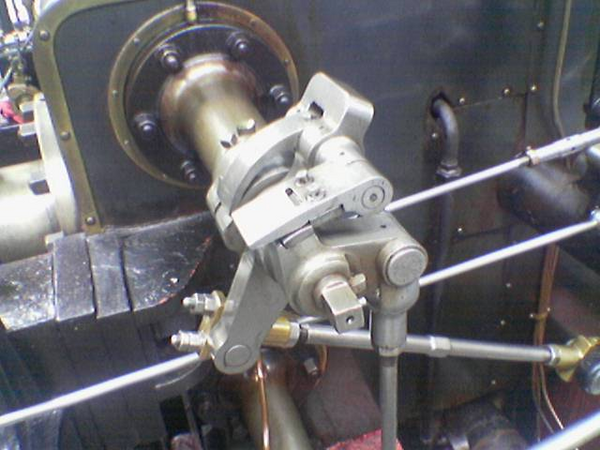
\includegraphics[width=.9\textwidth]{cnn/pre-sobel.png}
        \end{minipage}
        \begin{minipage}{0.4\textwidth}
            \centering
            \caption*{Sobel operator applied to the image}
            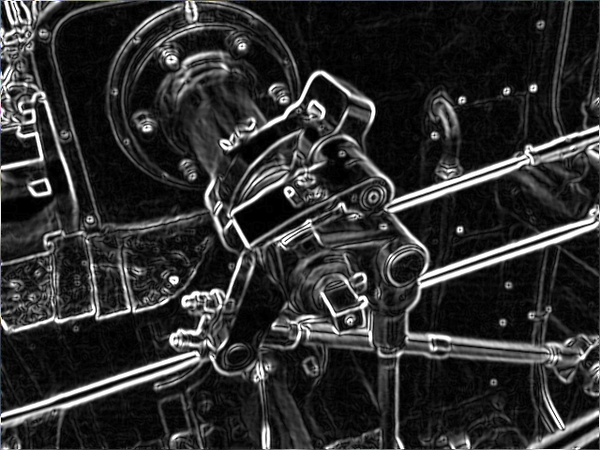
\includegraphics[width=.9\textwidth]{cnn/post-sobel.png}
        \end{minipage}

        \caption{Effect of the Sobel operator on an image}
    \end{figure}
\end{example}

These two examples show that kernels used in convolutional layers express meaningful transformations of the input, justifying their use in CNNs. For instance, one could hardcode different kernels (gaussian blur, Sobel operator, vertical/horizontal lines extraction) to extract interesting features from an image, and plug these features into an MLP to obtain an improved classifier compared to a basic, flattening MLP. We will see that instead, CNNs have learnable kernel weights, allowing the model to choose the kernels that it considers bests.

\subsubsection{Multiple kernels}
In Figure \ref{fig:one-kernel-layer}, we used simply one kernel to compute one activation map. In practice, we repeat this process multiple times: we consider a set (or \emph{bank}) of filters having different weights values, and for each kernel of the set, we compute its activation map.
\begin{figure}[H]
    \centering
    \begin{tikzpicture}
        % Input
        \node at (.8, 1.7) {Input image};
        \parallelepiped{(0, 0, 0)}{.5}{4}{3}{$3$}{$32$}{$32$}{blue!20}

        % Convolution Layer
        \draw[thick] (1.5, -1) -- ++ (2.25, 0);
        \node[rectangle,draw,thick,rounded corners] at (5, -1) {\begin{varwidth}{2.5cm}\centering Convolution Layer\end{varwidth}};
        \draw[thick, ->] (6.25, -1) -- ++ (2.25, 0);

        % Kernels
        \node at (5, -4.5) {6 kernels};
        \draw[thick, ->] (5.1, -2.5) -- ++ (0, 0.9);
        \parallelepiped{(3.8, -3, 0)}{.3}{1}{.75}{$3$}{$5$}{}{orange!40};
        \foreach \x in {4.3, 4.8, ..., 5.8} {
            \parallelepiped{(\x, -3, 0)}{.3}{1}{.75}{}{}{}{orange!40};
        }
        \parallelepiped{(6.3, -3, 0)}{.3}{1}{.75}{}{}{$5$}{orange!40};

        % Activation maps
        \node at (10.8, 1.7) {6 activation maps};
        \parallelepiped{(9, 0, 0)}{.2}{3.5}{2.75}{$1$}{$28$}{}{red!40};
        \foreach \x in {9.5, 10, ..., 11} {
            \parallelepiped{(\x, 0, 0)}{.2}{3.5}{2.75}{}{}{}{red!40};
        }
        \parallelepiped{(11.5, 0, 0)}{.2}{3.5}{2.75}{}{}{$28$}{red!40};
        \node at (10.7, -4.5) {$6\times28\times28$ output};
    \end{tikzpicture}
    \caption{Convolutional Layer using 6 kernels}
\end{figure}

Using a bank containing $C'$ filters, the output of the convolutional layer in an \emph{activation map} of dimension $C'\times (H - K + 1) \times (W - K + 1)$ representing for each pixel the convolution between the given kernel and the corresponding chunk of the image.

\begin{remark}[Biases in Convolutional Layers]
    Similarly to fully-connected layers, we often add to the activation map of each kernel a bias of size $1\times (H - K + 1) \times (W - K + 1)$. Those biases might me ommited in the rest of the chapter for the sake of simplicity.
\end{remark}

\subsubsection{Stacking convolutions}
Like previously introduced layers, convolutional layers can be stacked to form deep networks. The layer shapes need to match, in particular the output channels of a layer must match the input channels of the next layer, and the output height and width must match the next input height and width.
\begin{figure}[H]
    \centering
    \begin{tikzpicture}
        % Input
        \node at (.5, 1.9) {\begin{varwidth}{3cm}\centering Input image $3\times32\times32$\end{varwidth}};
        \parallelepiped{(0, 0, 0)}{.5}{4}{3}{$3$}{$32$}{$32$}{blue!20}

        % Convolution layer
        \draw[thick] (1.5, -1) -- ++ (.8, 0);
        \node[rectangle,draw,thick,rounded corners] at (3, -1) {Conv.};
        \draw[thick, ->] (3.7, -1) -- ++ (.8, 0);
        \node at (3, -.3) {$6\times3\times5\times5$};

        % First hidden layer
        \node at (6, 1.7) {\begin{varwidth}{3.5cm}\centering First hidden layer $3\times28\times28$\end{varwidth}};
        \parallelepiped{(5.75, 0, 0)}{1}{3.5}{2.5}{$6$}{$28$}{$28$}{red!40}

        % Convolution layer
        \draw[thick] (7, -1) -- ++ (.8, 0);
        \node[rectangle,draw,thick,rounded corners] at (8.5, -1) {Conv.};
        \draw[thick, ->] (9.2, -1) -- ++ (.8, 0);
        \node at (8.5, -.3) {$10\times6\times3\times3$};

        % Second hidden layer
        \node at (11.5, 1.5) {\begin{varwidth}{4cm}\centering Second hidden layer $3\times26\times26$\end{varwidth}};
        \parallelepiped{(11.5, 0, 0)}{1.3}{3.1}{2.1}{$10$}{$26$}{$26$}{green!20}

        % Convolution layer
        \draw[thick] (12.5, -1) -- ++ (.8, 0);
        \node[rectangle,draw,thick,rounded corners] at (14, -1) {Conv.};
        \draw[thick, ->] (14.7, -1) -- ++ (.8, 0);
        \node at (14, -.3) {$12\times10\times3\times3$};
    \end{tikzpicture}
    \caption{Stacking of 3 Convolutional Layers of correct shapes}
\end{figure}

However, stacking two convolution layers next to each other produces another convolutional layers, and do not add representation power. Therefore, we use the exact same solution as for linear classifiers: we introduce non-linear layers using activation functions in between convolutional layers.
\begin{figure}[H]
    \centering
    \begin{tikzpicture}
        % Input
        \node at (.5, 1.9) {\begin{varwidth}{3cm}\centering Input image $3\times32\times32$\end{varwidth}};
        \parallelepiped{(0, 0, 0)}{.5}{4}{3}{$3$}{$32$}{$32$}{blue!20}

        % Convolution layer
        \draw[thick] (1.2, -1) -- ++ (.35, 0);
        \draw[thick] (2.85, -1) -- ++ (.2, 0);
        \draw[thick, ->] (4.35, -1) -- ++ (.5, 0);
        \node[rectangle,draw,thick,rounded corners] at (2.2, -1) {Conv.};
        \node[rectangle,draw,thick,rounded corners] at (3.7, -1) {ReLU};

        % First hidden layer
        \node at (6, 1.7) {\begin{varwidth}{3.5cm}\centering First hidden layer $3\times28\times28$\end{varwidth}};
        \parallelepiped{(5.75, 0, 0)}{.8}{3.5}{2.5}{$6$}{$28$}{$28$}{red!40}

        % Convolution layer
        \draw[thick] (6.8, -1) -- ++ (.35, 0);
        \draw[thick] (8.45, -1) -- ++ (.2, 0);
        \draw[thick, ->] (9.95, -1) -- ++ (.5, 0);
        \node[rectangle,draw,thick,rounded corners] at (7.8, -1) {Conv.};
        \node[rectangle,draw,thick,rounded corners] at (9.3, -1) {ReLU};

        % Second hidden layer
        \node at (11.5, 1.5) {\begin{varwidth}{4cm}\centering Second hidden layer $3\times26\times26$\end{varwidth}};
        \parallelepiped{(11.5, 0, 0)}{1}{3.1}{2.1}{$10$}{$26$}{$26$}{green!20}

        % Convolution layer
        \draw[thick] (12.5, -1) -- ++ (.35, 0);
        \draw[thick] (14.15, -1) -- ++ (.2, 0);
        \draw[thick, ->] (15.65, -1) -- ++ (.5, 0);
        \node[rectangle,draw,thick,rounded corners] at (13.5, -1) {Conv.};
        \node[rectangle,draw,thick,rounded corners] at (15, -1) {ReLU};
    \end{tikzpicture}
    \caption{Adding ReLU layers in between Convolution Layers}
\end{figure}

\subsubsection{Spatial dimensions and Padding}
As stated previously, using an input of width $W$ with a filter of kernel size $K$, the output width is $W-K+1$. A problem with the approach is that features maps decrease in size with each layer. This creates an upper bound on the maximum number of layers that we can use for our model.

A solution to this is to introduce \emph{padding} by adding zeros around the border of the input. When the kernel will slide around the edges of the input, a part of the coefficients that it will consider in its convolution will be zeros.
\begin{figure}[H]
    \centering
    \begin{tikzpicture}
        \newcommand{\randint}{
            \pgfmathsetmacro{\temp}{random(0, 9)}
            \temp
        }
        \newcommand{\phant}{
            \makebox[0pt][l]{\footnotesize\,$\cdot$}\phantom{0}
        }

        \tikzstyle{number matrix}=[
            matrix of math nodes,
            nodes={
                minimum size=1em,
                outer sep=0pt,
                inner sep=0,line
                width=0.5pt,
            },
            nodes in empty cells,
            column sep=-0.5pt,
            row sep=-0.5pt
        ]

        \matrix [number matrix, nodes={
            append after command={
                \pgfextra{\draw[thick, dashed]
                ($(\tikzlastnode.north west)+(-0.3em,+0.3em)$)
                rectangle ($(\tikzlastnode.south east)+(0.3em,-0.3em)$);}
            }
        }] at (0, 0)
        {
            0 & 0 & 0 & 0 & 0 & 0 & 0 & 0 \\
            0 & 0 & 0 & 0 & 0 & 0 & 0 & 0 \\
            0 & 0 & 0 & 0 & 0 & 0 & 0 & 0 \\
            0 & 0 & 0 & 0 & 0 & 0 & 0 & 0 \\
            0 & 0 & 0 & 0 & 0 & 0 & 0 & 0 \\
            0 & 0 & 0 & 0 & 0 & 0 & 0 & 0 \\
            0 & 0 & 0 & 0 & 0 & 0 & 0 & 0 \\
            0 & 0 & 0 & 0 & 0 & 0 & 0 & 0 \\
        };

        \matrix [number matrix, nodes={
            append after command={
                \pgfextra{\draw[thick, fill=gray!30]
                ($(\tikzlastnode.north west)+(-0.3em,+0.3em)$)
                rectangle ($(\tikzlastnode.south east)+(0.3em,-0.3em)$);}
            }
        }] at (0, 0)
        {
            2 & 5 & \randint & \randint & \randint & \randint \\
            7 & 1 & \randint & \randint & \randint & \randint \\
            \randint & \randint & \randint & \randint & \randint & \randint \\
            \randint & \randint & \randint & \randint & \randint & \randint \\
            \randint & \randint & \randint & \randint & \randint & \randint \\
            \randint & \randint & \randint & \randint & \randint & \randint \\
        };

        \fill[color=blue, fill opacity=.4] (-8/3, 8/3) rectangle (-2/3, 2/3);

        % Dashed connections
        \draw[-, dashed] (-8/3, 8/3) -- (4, 1);
        \draw[-, dashed] (-2/3, 8/3) -- (6, 1);
        \draw[-, dashed] (-8/3, 2/3) -- (4, -1);
        \draw[-, dashed] (-2/3, 2/3) -- (6, -1);

        \draw[-, dashed] (4, 1) -- (8, 2);
        \draw[-, dashed] (6, 1) -- (26/3, 2);
        \draw[-, dashed] (4, -1) -- (8, 4/3);
        \draw[-, dashed] (6, -1) -- (26/3, 4/3);

        \matrix [number matrix, nodes={
            append after command={
                \pgfextra{\draw[thick, fill=orange, fill opacity=.6]
                ($(\tikzlastnode.north west)+(-0.3em,+0.3em)$)
                rectangle ($(\tikzlastnode.south east)+(0.3em,-0.3em)$);}
            }
        }] at (5, 0)
        {
            \randint & \randint & \randint \\
            \randint & 1 & 1 \\
            \randint & 0 & 2 \\
        };

        \fill[color=red, fill opacity=.5] (8, 2) rectangle (26/3, 4/3);
        \matrix [number matrix, nodes={
            append after command={
                \pgfextra{\draw[thick]
                ($(\tikzlastnode.north west)+(-0.3em,+0.3em)$)
                rectangle ($(\tikzlastnode.south east)+(0.3em,-0.3em)$);}
            }
        }] at (10, 0)
        {
            9 & \phant & \phant & \phant & \phant & \phant \\
            \phant & \phant & \phant & \phant & \phant & \phant \\
            \phant & \phant & \phant & \phant & \phant & \phant \\
            \phant & \phant & \phant & \phant & \phant & \phant \\
            \phant & \phant & \phant & \phant & \phant & \phant \\
            \phant & \phant & \phant & \phant & \phant & \phant \\
        };

        \node at (3.3, 0) {\Large *};
        \node at (6.9, 0) {\Large =};

        \node at (0, 3.2) {Input image with $(1, 1)$ padding};
        \node at (0, -3.2) {$6\times6 \longrightarrow 8\times8$};
        \node at (5, -1.5) {$3\times3$};
        \node at (10, 2.5) {Output image};
        \node at (10, -2.5) {$6\times6$};

    \end{tikzpicture}
    \caption{Adding padding around the input}
\end{figure}

\begin{remark}[Padding strategies]
    Even though we might imagine different padding strategies instead of always padding with zeros (for instance, nearest-neightbour padding, circular padding, random padding\dots), zero-padding seems to be both simple and effective in practice, and is the most commonly used strategy.
\end{remark}

Padding introduces an additional hyperparameter to the layer, $P$.
Using padding, the width of the output of the layer becomes:
\begin{equation}
    \label{eq:output-padding}
    W'=W-K+2P+1
\end{equation}
A common way to set the value of $P$ is to choose it such as the output have the same size as the input. This is achieved by taking $P=(K-1)/2$, called \emph{same-padding}. This is only possible if $K$ is odd, which is often the case in practice, since same-padding is often the expected behavior.

\subsubsection{Receptive Fields}
\begin{definition}[Receptive Field]
    The \emph{receptive field} of an output neuron is the set of neurons of the input of which the output neuron depends on.
\end{definition}

By essence, Fully-connected layers have a trivial notion of receptive field: an output neuron is connected to each input neuron, its receptive field is therefore the entire input.

Convolution layers are build in such a way that each element in the output simply depends on a receptive field of size $K$ (that is a square of area $K\times K$) in the input. As we stack convolutional layers after the others, each successive convolution adds $K-1$ to the receptive field size. After $L$ layers, the receptive field size is $1+L\times(K-1)$.

\begin{figure}[H]
    \centering
    \begin{tikzpicture}[scale=.9]
        \tikzstyle{custom width}=[line width=0.6mm]
        \tikzstyle{orange}=[color=orange]
        \tikzstyle{blue}=[color=RoyalBlue]
        \tikzstyle{green}=[color=SeaGreen]

        \draw[step=0.5] (0,0) grid (3.5,3.5);
        \node at (1.725, -.4) {Input};
        \draw[step=0.5] (3.99,0) grid (7.5,3.5);
        \draw[step=0.5] (7.99,0) grid (11.5,3.5);
        \draw[step=0.5] (11.99,0) grid (15.5,3.5);
        \node at (13.725, -.4) {Output};

        \draw[orange, custom width] (0,2) rectangle ++(1.5,1.5);
        \draw[orange, dashed, custom width] (1.5, 3.5) -- (4.5,3);
        \draw[orange, dashed, custom width] (1.5, 2) -- (4.5,2.5);

        \draw[orange, custom width] (2,0) rectangle ++(1.5,1.5);
        \draw[orange, dashed, custom width] (3.5, 1.5) -- (6.5,1);
        \draw[orange, dashed, custom width] (3.5, 0) -- (6.5,.5);

        \draw[blue, custom width] (4.5,1.5) rectangle ++(1.5,1.5);
        \draw[blue, dashed, custom width] (6,3) -- (9,2.5);
        \draw[blue, dashed, custom width] (6,1.5) -- (9,2);

        \draw[blue, custom width] (5.5,0.5) rectangle ++(1.5,1.5);
        \draw[blue, dashed, custom width] (7,1.5) -- (10,1.5);
        \draw[blue, dashed, custom width] (7,0.5) -- (10,1);

        \draw[orange, custom width] (4.5,2.5) rectangle ++(.5,.5);
        \draw[orange, custom width] (6.5,0.5) rectangle ++(.5,.5);

        \draw[green, custom width] (9,1) rectangle ++(1.5,1.5);
        \draw[green, dashed, custom width] (10.5,2.5) -- (13.5,2);
        \draw[green, dashed, custom width] (10.5,1) -- (13.5,1.5);

        \draw[blue, custom width] (9,2) rectangle ++(.5,.5);
        \draw[blue, custom width] (10,1) rectangle ++(.5,.5);

        \draw[green, custom width] (13.5,1.5) rectangle ++(.5,.5);
    \end{tikzpicture}
    \caption{Receptive field of an output neuron}
\end{figure}

This linear growth shows that by stacking enough layers, each output neuron will eventually have the entire input image in its receptive field. Nevertheless, this can be a problem in practice as we might need many layers for each output to depend on the whole image.

A solution to this problem is to downsample the image size inside the network. This can be done by adding another hyperparameter, \emph{stride}.

\subsubsection{Strided Convolution}
\begin{definition}[Stride]
    The hyperparameter \emph{stride} defines the number of pixels between two applications of the kernel.
\end{definition}
\begin{wrapfigure}{r}{0.4\textwidth}
    \centering
    \begin{tikzpicture}
        \newcommand{\randint}{
            \pgfmathsetmacro{\temp}{random(0, 1)}
            \temp
        }
        \fill[orange!60] (-2, -2) rectangle (2, 2);
        \matrix [
            matrix of math nodes,
            nodes={
                minimum size=1em,
                outer sep=0pt,
                inner sep=0,line
                width=0.5pt,
                append after command={
                    \pgfextra{\draw[thick]
                    ($(\tikzlastnode.north west)+(-0.3em,+0.3em)$)
                    rectangle ($(\tikzlastnode.south east)+(0.3em,-0.3em)$);}
                }
            },
            nodes in empty cells,
            column sep=-0.5pt,
            row sep=-0.5pt
        ]
        {
            \randint & \randint & \randint & \randint & \randint & \randint \\
            \randint & \randint & \randint & \randint & \randint & \randint \\
            \randint & \randint & \randint & \randint & \randint & \randint \\
            \randint & \randint & \randint & \randint & \randint & \randint \\
            \randint & \randint & \randint & \randint & \randint & \randint \\
            \randint & \randint & \randint & \randint & \randint & \randint \\
        };

        \draw[densely dashed, color=red, line width=1mm] (-2, 0) rectangle (0, 2);
        \draw[color=red, line width=1mm] (-2/3, 0) rectangle (4/3, 2);

        \draw[<->, color=red, very thick] (-2, 2.2) -- (-2/3, 2.2) node[above, pos=.5] {\bf stride};
    \end{tikzpicture}
    \caption{Effect of stride}
\end{wrapfigure}

Stride effectively downsamples the size of the image. Applying a convolution between an image of width $W$ and padding $P$ with a kernel of size $K$ and stride $S$ produces the following output dimension:
\begin{equation}
    \label{eq:output-stride}
    W'=\frac{W-K+2P}{S}+1
\end{equation}
Note that choosing $S=1$ in \eqref{eq:output-stride} gives the same result as \eqref{eq:output-padding}. Depending on the implementation, the result can be rounded up or down in the case where it is not an integer. Usually, all the parameters are chosen such that $S$ divides $W-K+2P$.

\subsection{Pooling Layers}
\subsubsection{Introduction}
Computer Vision, one of the most frequent use for CNNs, often deals with images of high quality, making downsampling an important task to drastically reduce the number of layers and the quantity of VRAM used by the model. We saw a first approach to downsampling embedded in Convolutional Layers, that is strided convolution. Pooling Layers are layers dedicated to downsampling, without learnable parameters.

Pooling layers work similarly to convolutional layers, using a mechanism of kernels. Nevertheless, instead of applying a convolution between some kernel and the image, the layer will apply a pooling function to the area of the input. This will produce an activation map with dimensions depending on the hyperparameters of the layer -- kernel size, padding and stride, the same as the parameters of a convolutional layer.

\begin{figure}[H]
    \centering
    \begin{tikzpicture}
        % Left block
        \parallelepiped{(0, 0, 0)}{2}{3}{2.5}{$64$}{$224$}{$224$}{orange!70};
        \parallelepiped{(-1.5, 0, 0)}{.15}{3}{2.5}{1}{}{}{blue!50};
        \draw[thick] (-2,0) -- ++(2, 0);

        % Right block
        \parallelepiped{(7, -.5, 0)}{2}{1.5}{1.5}{$64$}{$112$}{$112$}{orange!70};
        \parallelepiped{(5.5, -.5, 0)}{.15}{1.5}{1.5}{1}{}{}{blue!50};
        \draw[thick] (5,-.5) -- ++(2, 0);

        % Pooling arrow
        \draw[thick, ->] (1.5, -1.2) -- ++(2.2, 0) node[pos=.5, above] {Pooling};
        % Downsampling arrow
        \draw[thick, ->] (0.2, -6.5) -- ++(4.3, 0) node[pos=.5, above] {Downsampling};

        % Left image
        \draw[thick, ->] (-1.5, -3.8) -- ++(0,-1);
        \node at (-1.5, -6.5) {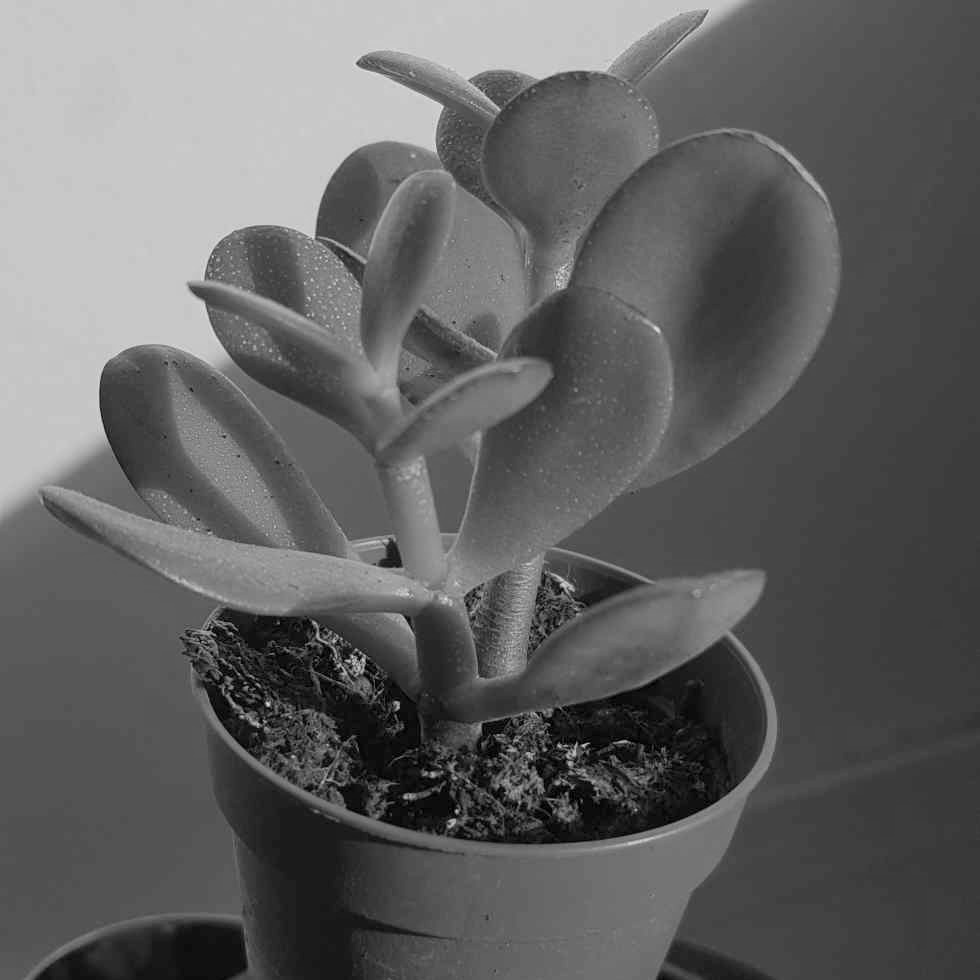
\includegraphics[width=80pt]{cnn/plante.jpg}};
        \node at (-3.3, -6.5) {$224$};
        \node at (-1.5, -8.2) {$224$};

        % Right image
        \draw[thick, <-] (5.5, -2.8) -- ++(0,-2.8);
        \node at (5.5, -6.5) {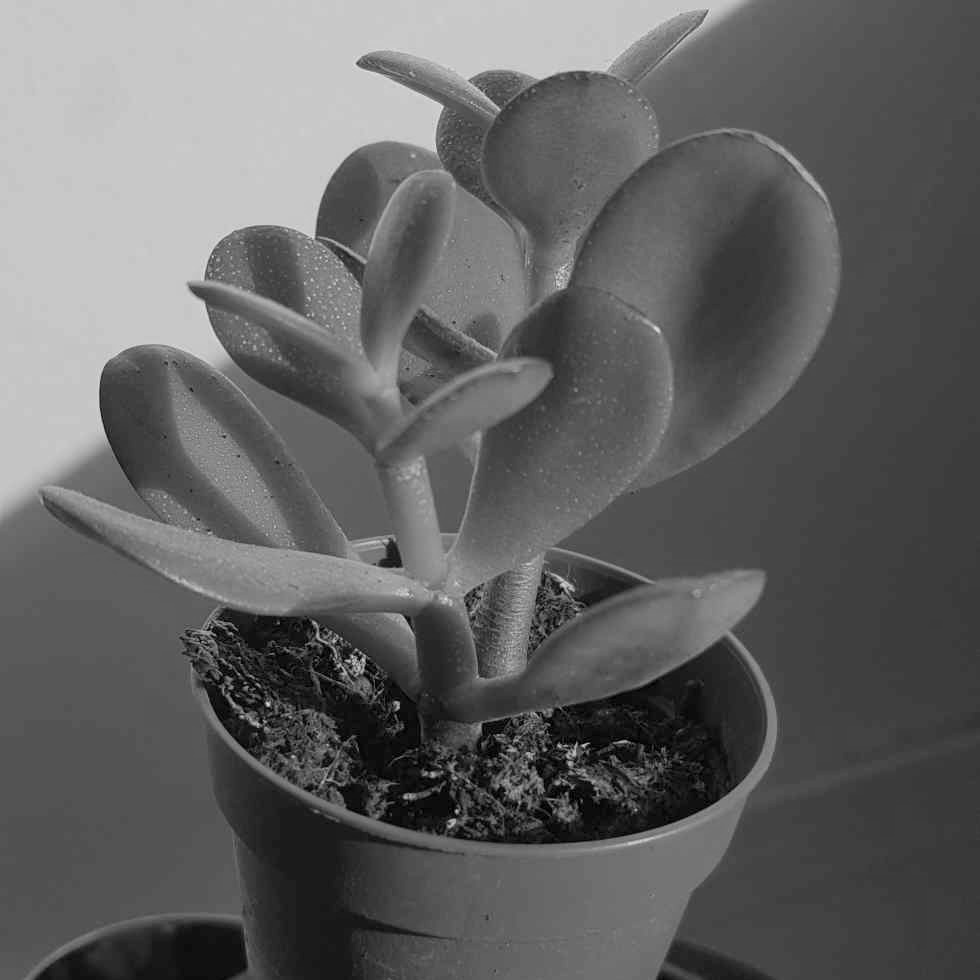
\includegraphics[width=40pt]{cnn/plante.jpg}};
        \node at (6.6, -6.5) {$112$};
        \node at (5.5, -7.5) {$112$};
    \end{tikzpicture}
    \caption{Behavior of a pooling layer}
\end{figure}
Another difference is that the operation is applied for each slice of the input volume. Choosing appropriate values for the hyperparameters (for instance $S\geq2$, \dots) allow to downsample the input without the need for learnable parameters.

\subsubsection{Max Pooling}
\begin{definition}[Max Pooling function]
    For $K\geq 1$, the \emph{Max Pooling function} of kernel size $K$ is:
    \begin{equation*}
        \begin{aligned}
            \textnormal{max}_P: \mathscr{M}_{K}(\R) &\longrightarrow \R\\
            (m_{i, j}) &\longmapsto \max_{i, j} m_{i, j}
        \end{aligned}
    \end{equation*}
\end{definition}

A \emph{Max Pooling} layer applies the Max Pooling function to each location of size $K\times K$ in each slice of the input volume. We often choose the same kernel size as the slide (that is $K=S$) to avoid recovering twice the same pixel value. In this setting, it is equivalent to spliting each input channel into non-overlapping regions of size $K\times K$, from which are extracted the maximum value of the section and stored in the output channel.

Max Pooling has some advantages over convolutional layers with stride: it does not involve learnable parameters, reducing the computational cost, but also introduces translational invariance to small spatial shifts. Indeed, if the position of a specific maximum pixel is moved slightly, we might intuitively think that it will stay the maximum of its region, making the model robust to small translations.

\subsubsection{Average Pooling}
\begin{definition}[Average Pooling function]
    For $K\geq 1$, the \emph{Average Pooling function} of kernel size $K$ is:
    \begin{equation*}
        \begin{aligned}
            \textnormal{avg}_P: \mathscr{M}_{K}(\R) &\longrightarrow \R\\
            (m_{i, j}) &\longmapsto \frac{1}{K^2}\sum_{i=1}^K \sum_{j=1}^K m_{i, j}
        \end{aligned}
    \end{equation*}
    It simply returns the average of the matrix coefficients.
\end{definition}

Average Pooling works exactly the same as Max Pooling, but applying $\textnormal{avg}_P$ as a pooling function instead of $\textnormal{max}_P$.

\subsection{A full CNN example: LeNet-5}
Now that we have these different types of layers, we can stack them together to create a full CNN architecture. A classic model often fits the following architecture:
\begin{equation*}
    (\texttt{Conv, ReLU, Pooling})^{N_1} \rightarrow \texttt{Flatten} \rightarrow (\texttt{Linear, ReLU})^{N_2} \rightarrow \texttt{Linear}
\end{equation*}

As an example, we will take the 1998 model \emph{LeNet-5}:
\begin{figure}[H]
    \centering
    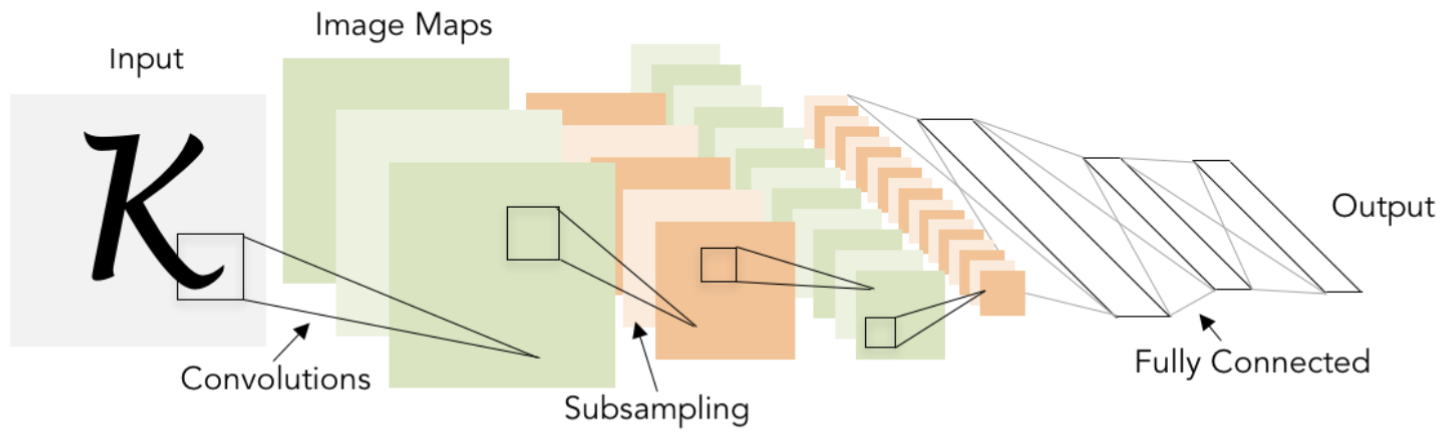
\includegraphics[width=0.8\textwidth]{cnn/lenet-5.png}
    \caption{LeNet-5 architecture}
\end{figure}
The first blocks of Convolutional and Pooling layers progressively decrease the spatial size of the input, while increasing the number of channels: the total volume of the input is preserved.

\subsection{Normalization}
\label{subseq:normalization}
Deep convolutional neural networks are described previously can be extremly effective when trained; nevertheless, they are also very difficult to train, and we need to properly prepare data for the descent to converge.

A recent solution to ease the training is to add \emph{normalization layers} in the network.

\subsubsection{Batch Normalization}
The idea of Batch Normalization is to normalize the outputs of a layer, often by giving the output a zero mean and unit variance. This improves optimization by guaranteeing that a layer always receive similar data from the previous layer's output. Indeed, while training, the distribution of the output of a layer might change, which tends to increase the complexity of the learning process. In contrast, the output of a batch normalization layers always has the same mean and variance; therefore, the next layer can always \say{see} the same input data distribution, improving convergence.

Normalizing batches of activations can simply be implemented using the following formula:
\begin{equation*}
    \hat{x}^{(k)} := \frac{x^{(k)} - \E[x^{(k)}]}{\sqrt{\V[x^{(k)}]}}
\end{equation*}
Hopefully, this is a differentiable function, and can therefore be seen as any other layer in the network, and implement its backward gradient.

\subsubsection{Batch Normalization in practice}
Consider a fully-connected setup, in which we have a batch $x$ consisting of $N$ inputs, each of size $D$. We will use the $N$ batch samples to compute the empirical mean for each of the element of the $D$-shaped vector:
\begin{equation*}
    \mu_j := \frac{1}{N}\sum_{i=1}^N x_{i, j}
\end{equation*}
which gives us a vector $\mu$ of size $D$. Similarly, the standard deviation of the batch can be computed element-wise:
\begin{equation*}
    \sigma_j^2 := \frac{1}{N}\sum_{i=1}^N (x_{i,j}-\mu_j)^2
\end{equation*}
giving us a vector $\sigma$ of size $D$ as well. Finally, each element of the batch $x$ is normalized, giving us $\hat{x}$:
\begin{equation*}
    \hat{x}_{i,j} := \frac{x_{i,j}-\mu_j}{\sqrt{\sigma^2_j+\epsilon}}
\end{equation*}
The small constant $\epsilon$ is added at the denominator to avoid diving by zero when the standard deviation is null.

In practice, zero mean and unit variance can be too hard of a constraint on the network. We prefer to add learnable scale and shift parameters $\gamma$ and $\beta$ of size $D$, allowing the network to choose what mean and variance it wants for the next layer. The acutal output is therefore $y$, defined by:
\begin{equation*}
    y_{i,j} := \gamma_j\hat{x}_{i,j}+\beta_j
\end{equation*}
Note that learning $\gamma=\sigma$ and $\beta=\mu$ recovers the identity function, making the network able to bypass the normalization layer if it is not needed.

An important note is that batch normalization introduces dependence on the minibatches: previously, each image in the input batch was handled independently of the others, which is not the case anymore with batch normalization. We cannot do this at test time, since it would not guarantee the reproducibility of classification, and more importantly, it would be a security breach to make each classification depend on the other inputs. To avoid this, batch normalization layers behave differently during training and testing. During training, the layer normalizes the batches as described before, while maintaining the empirical mean and variance of the inputs, $\mu$ and $\sigma$. These empirical vectors learned during training are then treated as constants and used during testing to normalize the test inputs.

Hence, at test time, the normalization layer performs the following operation:
\begin{equation*}
    y = \gamma\cdot\frac{x-\mu}{\sigma}+\beta
\end{equation*}
Another interesting property of this method is that during testing, the batch normalization layer becomes a linear operator. Therefore, it can be fused with the previous fully-connected or convolutional layer. For instance, if the previous layer is a fully-connected, its weight matrix and bias vector can be modified using the four parameters of the normalization layer (learned mean and variance, and empirical mean and variance). Performing this operation guarantees that the batch normalization layer does not add any inference time.

\subsubsection{Batch Normalization for Convolutional Networks}
For fully-connected layers, the batch dimension is:
\begin{equation*}
    x: N\times D
\end{equation*}
Therefore, the batch normalization parameters are the following:
\begin{equation*}
    \begin{cases*}
        \mu, \sigma: 1\times D & (empirical mean and standard deviation)\\
        \gamma, \beta: 1\times D & (learned mean and standard deviation)
    \end{cases*}
\end{equation*}

This needs to be adapted for convolutional layers, but remains very similar. The batch dimension is:
\begin{equation*}
    x: N\times C\times H\times W
\end{equation*}
Instead of averaging only over the batch elements, we will also average over both spacial dimensions. This means that we will take for each channel the average and standard deviation taking into account all the pixels of all the images in the batch. Therefore, the batch normalization parameters are the following:
\begin{equation*}
    \begin{cases*}
        \mu, \sigma: 1\times C\times 1\times 1 & (empirical mean and standard deviation)\\
        \gamma, \beta: 1\times C\times 1\times 1 & (learned mean and standard deviation)
    \end{cases*}
\end{equation*}
which can also be seen as vectors of size $C$; it is nevertheless more convenient to see them in tensor form, $1\times C\times 1\times 1$.

\subsubsection{Advantages and downsides of batch normalization}
As stated previously, adding batch normalization in neural networks allows for models to train much faster, while adding no overhead at testing time when placed after fully-connected or convolutional layers.

Not only the models converge quicker at fixed learning rate, but it also stabilizes the model even with higher learning rates, allowing shorter training times without the risk of divergence.

While they are widely used in practice, normalization layers also come with downsides: the reason of the effectiveness of batch normalization is not well-understood theoretically, and it introduces complex code because of the distinction between training and testing. This is actually a very common source of bugs in projects: one have to remember to change the mode from training to testing.

Finally, batch normalization is not always appropriate: some very unbalanced data sets might not fit appropriately with batch normalization, and this can reduce the performance of the model. This depends highly on the application: for computer vision, batch normalization is most of the time suitable.

\subsubsection{Layer and Instance normalizations}
A variant to batch normalization, called \emph{layer normalization}, has be proposed. It aims at unifying the behavior of the normalization layer at training and testing time. This guarantees, even at training time, the independence between elements of one batch. The idea is to normalize the input in the layer direction instead of the batch direction. For a fully-connected layer with batch dimension:
\begin{equation*}
    x:N\times D
\end{equation*}
the layer normalization parameters become:
\begin{equation*}
    \begin{cases*}
        \mu, \sigma: N\times 1 & (empirical mean and standard deviation)\\
        \gamma, \beta: \;\,1\times D & (learned mean and standard deviation)
    \end{cases*}
\end{equation*}
This kind of normalization is currently used in recurrent neural networks (RNNs) and transformers.

The equivalent of layer normalization for convolutional layers is called \emph{instance normalization}: similarly, instead of averaging over both the batch and spatial dimensions, we will only normalize over the spatial dimensions. For a convolution layer with batch dimension:
\begin{equation*}
    x: N\times C\times H\times W
\end{equation*}
the layer normalization parameters become:
\begin{equation*}
    \begin{cases*}
        \mu, \sigma: N\times C\times 1\times 1 & (empirical mean and standard deviation)\\
        \gamma, \beta: \;\,1\times C\times 1\times 1 & (learned mean and standard deviation)
    \end{cases*}
\end{equation*}

\begin{figure}[H]
    \centering
    \begin{tikzpicture}[scale=1.3]
        \node at (.6, 2.4) {\bf Batch Norm};
        \node[rotate=90] at (-1.2,0.1) {H, W};
        \node at (0,-1.2) {C};
        \node at (1.7,-0.7) {N};

        \node at (4.6, 2.4) {\bf Layer Norm};
        \node[rotate=90] at (4-1.2,0.1) {H, W};
        \node at (4+0,-1.2) {C};
        \node at (4+1.7,-0.7) {N};

        \node at (8.6, 2.4) {\bf Instance Norm};
        \node[rotate=90] at (8-1.2,0.1) {H, W};
        \node at (8+0,-1.2) {C};
        \node at (8+1.7,-0.7) {N};


        \foreach\x in {0, 0.35, ..., 2.1} {
        \foreach\y in {0, 0.35, ..., 2.1} {
        \foreach\z in {0, 0.35, ..., 2.1} {
            % Batch Norm
            \pgfmathparse{\x>=1.75}
            \ifnum\pgfmathresult=1
                \parallelepiped{(\x, \y, \z)}{.3}{.3}{.3}{}{}{}{NavyBlue!100}
            \else
                \parallelepiped{(\x, \y, \z)}{.3}{.3}{.3}{}{}{}{gray!30}
            \fi


            % Layer Norm
            \pgfmathparse{\z>=1.75}
            \ifnum\pgfmathresult=1
                \parallelepiped{(4+\x, \y, \z)}{.3}{.3}{.3}{}{}{}{NavyBlue!100}
            \else
                \parallelepiped{(4+\x, \y, \z)}{.3}{.3}{.3}{}{}{}{gray!30}
            \fi


            % Instance Norm
            \pgfmathparse{\x>=1.75 && \z>=1.75}
            \ifnum\pgfmathresult=1
                \parallelepiped{(8+\x, \y, \z)}{.3}{.3}{.3}{}{}{}{NavyBlue!100}
            \else
                \parallelepiped{(8+\x, \y, \z)}{.3}{.3}{.3}{}{}{}{gray!30}
            \fi
        }}}
    \end{tikzpicture}
    \caption{Visualization of the different types of normalization. The blue squares represent the parts normalized together.}
\end{figure}